\chapter{Návrh systému}
\label{navrh}
Cílem této kapitoly je podívat se na vytvářený systém z abstraktnějšího pohledu a prozkoumat jednotlivé akce, které bude systém provádět. Akcí bude několik, proto systém bude rozdělen do logických celků, které obstarávají určitou část procesu analýzy. Na každou z~těchto částí jsou kladeny určité požadavky, které musí být splněny. 

Systém je navrhován postupně, podle jednotlivých kroků analýzy. Prvním krokem je obstarání dat, druhým je jejich uložení, dále pak jejich zpracování a analýza. Informace získané analýzou poté budou prezentovány. 

\section{Získání dat}
Jak již bylo popsáno v teoretickém rozboru (kapitola \ref{stahovani}), data jsou pro tento systém velice důležitá. Dále bylo rozebráno, že budou potřeba data pro trénování i samotnou analýzu. Trénovací datová sada by měla ideálně obsahovat anotace hledaných odpovědí klasifikátoru. Recenzí bude potřeba co nejvíce a při jejich větším počtu nepřipadá manuální anotace (označování) v úvahu. Z tohoto důvodu by bylo ideální najít zdroj recenzí, kde jsou jednotlivé recenze již anotovány. Možností jejich získání je hned několik, záleží na konkrétním zvoleném zdroji. Nejpohodlnějším způsobem získávání recenzí by bylo za využití \emph{API} dané webové stránky, další možností je využít jednu z popsaných technik extrakce dat v~kapitole~\ref{stahovani}. 

Možných zdrojů dat je velké množství, lidé dnes využívají pro sdíleních svých názorů sociální média, blogy, fóra, specializované stránky pro recenze a další. 

Získávání dat ze sociálních médií je pravděpodobně nejjednodušší, protože obvykle nabízí \emph{API}. Na druhou stranu data na sociálních médiích neobsahují požadované anotace, poměrně často bývají irelevantní a kvůli zvyšujícímu se soukromí na těchto platformách se informace stávají nepřístupnými. 

Dále by se daly využít již vytvořené datové sady. Komunita věnující se zpracování přirozeného jazyka je velice aktivní po celém světě, takže se dá nalézt již anotovaná datová sada téměř v jakémkoli jazyku. Tento přístup by se dal využít k počátečnímu natrénování klasifikátorů, systém by však měl být schopný automaticky a pravidelně stahovat nové recenze, aby zůstal aktuální. 

Nejlepším zdrojem dat tedy nejspíš bude některá z webových stránek specializujících se na filmové recenze. Tyto stránky splňují všechna dříve zmíněná kritéria. Navíc velké platformy obvykle  mají i vlastní \emph{API}, které by zjednodušilo získávání recenzí. 

\subsection{Extrahované informace}
Nezávisle na zdroji recenzí, ze získávaných příspěvků bude pro úspěšnou analýzu nutnost získávat určité informace. Nejdůležitější je samozřejmě samotný text recenze, dále je však potřeba číselné hodnocení autora pro následné porovnání hodnot při trénovaní klasifikátorů. Další důležitou informací je cíl dané recenze (tedy film, kterého se recenze týká). Uživatelské jméno autora se dá využít k případné identifikaci této recenze, popřípadě k přiřazení váhy k~recenzi na základě toho, kdo danou recenzi napsal. Datum vytvoření recenze bude užitečné pro sledování postupné změny názorů v čase. Poslední získávanou informací by měla být webová stránka, ze které byla recenze stažena. Tato informace je důležitá pro následné nalezení recenze a pro identifikaci jazyka recenze (systém by měl pracovat pro český i~anglický jazyk).

\subsection{Ukládání dat}
Zmíněno v teorii (kapitola \ref{ukladani}), k uchování získaných dat je více možností. Tento systém by však nejlépe fungoval s využitím relačního databázového systému. Důvodem je strukturovanost extrahovaných dat (bude stačit ukládání do tabulek, není tedy potřeba NoSQL databáze). Na druhou stranu ukládání do souborů (v serializačním formátu) by nebylo velice moudré, protože je předpokládané velké množství recenzí a k uloženým datům bude pravděpodobně přistupovat více částí systému najednou. Velké soubory se pomalu zpracovávají a není možné s nimi pracovat z několika míst najednou. 

\section{Analýza dat}
Po získání a uložení dat v systému navazuje jejich analýza. Data by měla být ukládána ve své původní formě, tedy neupravené, pro zachování co nejvíce informací. Před samotnou analýzou by se však měla předzpracovat využitím technik popsaných v kapitole \ref{predzpracovani}. Předzpracování pomáhá systému zvýšit jeho přesnost. 

Nejvyšších přesností dosahují metody klasifikace založené na strojovém učení, z tohoto důvodu bude tato část systému rozdělena na část pro trénování klasifikátoru a část využívající natrénovaný klasifikátor. 

Recenze bych analyzoval na úrovni dokumentu a úrovni aspektu. Na úrovni dokumentu by byla prováděna polaritní analýza (pozitivní / negativní polarita), dále pak analýza míry této pozitivity (jedna až pět, nebo jedna až deset hvězd). Dále by mohla být prováděna analýza na úrovni aspektu pro získání detailnějších informací z recenze. Ke zjištění jaké aspekty budou analyzovány bude potřeba prozkoumat uživatelské recenze a zjistit o čem uživatelé nejčastěji píší. Pro aspektovou analýzu bude oproti ostatním nutné ručně anotovat recenze, nalézt již vytvořenou datovou sadu se mi asi nepodaří.

Analýzu je možné provádět množstvím metod, chtěl bych jich tedy vyzkoušet několik a~porovnat jejich výsledky. 

Výsledky analýzy by se měli opět ukládat do relační databáze pro jejich následné zpracování a zobrazení.

\section{Zpracování a vizualizace výsledků}
Pouhý soupis výsledků jednotlivých analýz by toho moc neprozradil. Je tedy vhodné výsledky agregovat a poté je zobrazit například grafem. K tomuto bych využil webové rozhraní z důvodu pohodlí uživatele. Nemusí nic stahovat ani instalovat, může se na stránky podívat téměř na jakémkoliv zařízení a uživatelé by si například mohli vytvořit vlastní účty.

Jednotlivé recenze a jejich výsledky bude samozřejmě nutné seskupit podle filmu, kterého se týkají. Uživatel poté může vyhledávat daný film, nebo procházet žebříček těchto filmů podle výsledných hodnot analýz. Dále by mohly být sledovány různé trendy titulů (popularita žánrů, jestli jsou populárnější filmy či seriály a podobně). 

\section{Výsledný systém}
Jednotlivé části systému by spolu měly komunikovat dle obrázku \ref{schema}.

\begin{figure}[!htb]
\label{schema}
\centering
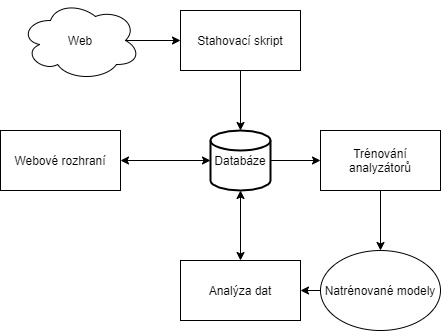
\includegraphics[width=\textwidth/2]{system_diagram.png}
\caption{Architektura navrhovaného systému. Jednotlivé části budou ovládány nástrojem pro plánování úloh.}
\end{figure}


\chapter{Implementace systému}
\label{implementace}
%\todo{INFORMACE VS DATA??, MUZU TAKHLE POUZIVAT?}
%\todo{OPRAVIT SLOVA TRCICI MIMO TEXT}
V této kapitole popisuji implementaci dříve definovaného systému. 
Systém je rozdělen do následujících částí:  

\begin{itemize}
  \item Stahování potřebných dat.
  \item Databáze.
  \item Trénování analyzátorů.
  \item Analýza sentimentu.
  \item Rozhraní pro zobrazení výsledků analýzy.
\end{itemize}

Pro každou z těchto částí je věnována samotná podkapitola. Při popisu každé z částí jsou nejprve prozkoumány možnosti řešení, které byly brány při v potaz a následuje popis výsledné implementace. 

Převážná většina systému je vytvořena v jazyku Python verze 3.6.9. Je využito několik pomocných skriptů pro bash. Výsledky analýzy jsou uživateli zobrazovány v prohlížeči za použití webového aplikačního rámce Django.
Systém běží na školním serveru \emph{Athena1} a je implementován pro češtinu i angličtinu. 

Protože je na systém požadavek pravidelné aktualizace dat, skripty pro stahování, zpracování dat a sémantickou analýzu je možné spouštět manuálně i automaticky. Postupně se tedy zvětšuje počet uložených recenzí v databázi. Tyto recenze jsou poté (opět automaticky) analyzovány natrénovanými klasifikátory. Natrénování klasifikátorů se dělá manuálně.

Automatické spouštění všech skriptů je prováděno pomocí plánovače úloh \emph{Cron}. Úlohy plánovače (takzvané \emph{Cronjobs}) jsou zapisovány do souboru zvaném \emph{Crontab} a mají následující formát:
\begin{center}
minuta[0-59] hodina[0-23] den měsíce[1-31] měsíc[1-12] den týdne[0-6] příkaz ke spuštění
\end{center}
%\todo{Popsat jak přesně funguje cron? musel bych najít na netu}

Namísto konkrétních čísel je možné využít znak hvězdičky, který zastupuje každou instanci (každou minutu, každou hodinu a podobně).
Z toho vyplývá že \emph{Cron} umožňuje spouštění jednou v konkrétní čas, ale i pravidelně.

\emph{Cron} nespouští přímo požadovaný python skript, ale jeden z dříve zmiňovaných bash skriptů. Tento bash skript nejprve zapne vývojové \emph{Conda} prostředí obsahující všechny systémem používané knihovny a potom až daný python skript.

Většina skriptů tvořících tento systém nějakým způsobem pracuje s daty, potřebují tedy přístup k nějakému úložišti dat. 
\clearpage
\pagebreak
Pro ukládání dat jsou podle potřeby využity:
\begin{itemize}
    \item Lokální soubory, formátu JSON nebo prostého textu.
    \item PostgreSQL databáze.
    \item SQLite databáze.
\end{itemize}

 

\section{Stahování dat}
Původně měli být zdroje dat Facebook a Twitter.
To se ovšem ukázalo jako ne tím nejlepším řešením, protože data ze sociálních sítí nebývají příliš kvalitní. Obě platformy mají navíc limitovaný přístup k datům a chybí zde číselné ohodnocení od autora.

Rozhodl jsem se tedy využít weby pro recenze filmů, kde jsou příspěvky relevantnější (uživatelé více vyjadřují svůj názor) a jsou dostupná číselná hodnocení od uživatelů. Díky číselnému hodnocení nemusí být texty recenzí manuálně anotována a hodnocení může být použito jako referenční výsledek pro trénování analyzátorů.
Toto řešení není úplně ideální, protože uživatelé občas dají pozitivní hodnocení (celkově se jim film líbil) a do textu recenze napíší všechny chyby filmu (určité části nebo detaily, které se jim nelíbily). Tohle by mohlo analyzátor při trénování zmást. Ideální by asi bylo data překontrolovat a hodnocení podle obsahu textu změnit. Dat je však tolik, že tohle není možné provést.


Zdroji dat se tedy staly weby \emph{csfd.cz}, \emph{fdb.cz}, \emph{rottentomatoes.com} a \emph{imdb.com}.
Pro získání dat z webových portálů jsem se pokusil získat přístup k jejich API, žádný z webů mi však nevyhověl (portál rottentomatoes.com má pro tento účel dotazník). 
Ke stažení recenzí z~daných webových stránek  tedy byly vytvořeny skripty využívající \emph{web scraping}. Každý portál má svůj vlastní skript. 

Všechny skripty pro stahování recenzí (kromě toho pro čsfd) mají společnou třídu \emph{Database\_manager} v souboru \emph{database\_manager.py}. Tato třída má na starost práci s PostgreSQL databází. Databáze běží na školním serveru \emph{Athena1}. Třída zajišťuje připojení a~přihlášení k databázi a implementuje několik funkcí pro dotazy a ukládání dat.

Stahování dat se spouští třídou \emph{Data\_downloader} v souboru \emph{data\_downloader.py}. Tato třída pouze podle nastavení v souboru \emph{config.py} spouští jeden stahovací skript za druhým.

Detailně jsou jednotlivé způsoby stahování dat popsány v následujících podkapitolách. 


\subsection{Stahování z ČSFD}

Stahování z této webové stránky je implementováno třídou \emph{Web\_scraper\_csfd} v souboru \emph{web\_scraper\_csfd.py}. Webové stránky \emph{csfd.cz} jsou celé implementovány staticky (nevyužívají JavaScript pro doplňování obsahu stránky). Z tohoto důvodu je stahování prováděno za využití knihovny \emph{urllib}, která umožňuje zasílat HTTP požadavky. Tato knihovna je implicitně součástí Python distribuce. Po získání HTTP odpovědi serveru jsou data zpracována pomocí knihovny \emph{BeautifulSoup} verze 4.8.2. Knihovna umožňuje procházet stromovou strukturou HTML dokumentu. 
Pro extrakci hledaných dat je nutné si nejprve projít strukturu stránky. Nejpohodlnější je využít funkci \uv{Prozkoumat}, kterou má každý webový prohlížeč a zjistit kde se ve stromové struktuře data nachází. Podle toho pak stačí využít vyhledávací funkce knihovny \emph{BeautifulSoup}. Možné je vyhledávat například podle názvu HTML značky, jejího id nebo třídy (class). Možností je samozřejmě více, pro detail má knihovna dokumentaci\footnote{\url{https://www.crummy.com/software/BeautifulSoup/bs4/doc/}}.

K vytvoření datové sady pro trénování analyzátorů i následnou analýzu jsou ke každé recenzi získávány následující informace:
\begin{itemize}
    \item Název titulu, ke kterému se recenze vztahuje.
    \item Text recenze.
    \item Hodnocení uživatele, na čsfd může uživatel hodnotit nula (odpad!) až pěti hvězdičkami, hodnota je před uložením normalizována na hodnotu mezi nulou a jedničkou.
    \item Identifikační číslo uživatele.
    \item Datum zveřejnění recenze.
\end{itemize}

Stahování nebylo možné provádět přímo na školním serveru \emph{Athena1}, protože po odeslání požadavku ze školního serveru na webový server se vždy vrátilo chybové hlášení. Z tohoto důvodu byl skript spouštěn na mém osobním počítači. 

K databázi na školním serveru se z venkovní sítě nedá připojit. Z tohoto důvodu byla na osobním počítači použita databáze SQLite. Databáze byla použita pro zaznamenávání již stažených příspěvků, aby skript nestáhl jeden příspěvek několikrát. Tabulka těchto záznamů má dva sloupce. Jeden pro název titulu a jeden pro identifikační číslo autora recenze. Předpokladem je, že každý uživatel napíše maximálně jednu recenzi ke každému titulu. 


Princip algoritmu pro stahování dat je následující. Nejprve se skript připojí k SQLite databázi pomocí třídy \emph{Database\_manager\_csfd}. Poté je zavolána funkce \emph{download\_all}, která započne stahování. Algoritmus využívá postupně vzrůstajícího identifikačního čísla uživatelů. Identifikační číslo uživatele od kterého má skript začít stahovat je nastavováno manuálně pro lepší kontrolu nad skriptem (alternativně by se mohlo číslo nastavit podle posledního záznamu v databázi). 
Postupně se tedy přičítá číslo aktuálního uživatele a prochází se odkazy následujícího formátu:
\begin{center}
    https://www.csfd.cz/uzivatel/<identifikační číslo uživatele>
\end{center}

Přijetím odpovědi serveru se zjistí, jestli účet uživatele s daným identifikačním číslem existuje. Pokud byl účet smazán, vrátí se chybová odpověď. Algoritmus si zaznamenává počet po sobě jdoucích chybových odpovědí. Pokud tato hodnota překročí určitou mez, stahování končí, protože algoritmus došel na konec seznamu identifikačních čísel uživatelů (identifikační čísla ještě nikdo nepoužívá). 

Pokud se od serveru vrátí pozitivní odpověď, přejde se do komentářové sekce uživatele. Postupně se prochází všechny komentáře daného uživatele a stahují se dříve zmiňované informace. Identifikační číslo uživatele a název komentovaného titulu se porovná se záznamy v SQLite databázi. Pokud takový záznam ještě neexistuje, tak se v databázi vytvoří a~informace se uloží. V opačném případě se informace zahodí. 
Stažená data jsou ukládána do lokálního souboru ve formátu JSON a později vložena do databáze na školním serveru. K uložení dat do školní databáze se používá pomocný skript \emph{upload\_csfd.py}. Na školním serveru jsou recenze ukládány do tabulky \emph{reviews}. 



\subsection{Stahování z FDb}
Implementováno třídou \emph{Web\_scraper\_fdb} v souboru \emph{Web\_scraper\_fdb.py}. Stejně jako\linebreak webové stránky čsfd jsou i tyto implementovány plně staticky, využívají se tedy stejné\linebreak nástroje (\emph{urllib} a \emph{BeaurifulSoup}). Stránky samozřejmě mají jinou strukturu než čsfd, proto je nutné je také projít (využitím nástroje \emph{Prozkoumat}) a vyhledat všechny důležité elementy HTML dokumentu. 

Seznam získávaných informací se oproti tomu z čsfd liší pouze v použití uživatelských jmen namísto identifikačních čísel.

Na rozdíl od skriptu pro čsfd, tento byl spouštěn na školním serveru. Byla tedy využita školní PostgreSQL databáze. K připojení a provádění akcí s databází je využita již zmiňovaná třída \emph{Database\_manager}. Pro záznamy již stažených recenzí (aby se jedna recenze nestáhla několikrát) je využita tabulka s názvem \emph{users\_fdb}, která funguje stejným způsobem jako SQLite databáze pro čsfd. Výsledné informace o recenzích jsou přímo ukládány do tabulky \emph{reviews}. 

Algoritmus funguje velice podobným způsobem jako při stahování z čsfd. Hlavním rozdílem je způsob procházení stránky (důvodem je samozřejmě jiná struktura stránek). 

Dalším rozdílem je postupné procházení uživatelů, které v tomto případě nevyužívá identifikačního čísla. Uživatelé i zde identifikační čísla mají a odkazy na uživatelské účty by se daly procházet stejným způsobem jako u čsfd. Stránky však při neexistenci uživatelského účtu s daným identifikačním číslem neodpoví chybovým hlášením. Namísto toho přesměrovávají na hlavní stránku (fdb.cz). Z tohoto důvodu jsou uživatelé nejprve vyhledáni v~žebříčku uživatelů a až poté se stahují jejich příspěvky.



\subsection{Stahování z Rotten Tomatoes}
Provádí třída \emph{Web\_scraper\_rottentomatoes} v souboru \emph{Web\_scraper\_rottentomatoes.py}.

Stránky jsou pouze částečně statické. 
Stahování dynamických stránek je mnohem pomalejší, protože se musí využít prohlížeče pro jejich vykreslení. Z tohoto důvodu jsem se rozhodl stahovat pouze statickou část stránek. Využité knihovny a základní postup procházení stránek je tedy pořád stejný. Stahování dynamických stránek jsem využil až pro stránky imdb, kde je u každého titulu mnohem více recenzí a tak se čekaní na načtení stránek více vyplatí. Například pro film Joker je na rotten tomatoes 137 000 hodnoceni, na imdb je to 821 000. Do těchto počtů jsou započítána i hodnocení bez napsání textu recenze, ale dá se předpokládat že na obou platformách komentuje stejné procento lidí. Stránky rotten tomatoes nezobrazují počet napsaných recenzí, proto bylo porovnání provedeno takto.

Statická část rotten tomatoes obsahuje top 100 filmů pro každý ze 17ti žánrů. Na této platformě jsou uživatelé rozdělení do dvou kategorií. Jedna kategorie jsou \emph{Audience} (tedy obecenstvo), což jsou obyčejní uživatelé této platformy. Druhou kategorií jsou \emph{critics} (tedy kritici), toto jsou uživatelé schválení platformou jako důvěryhodní. Stahovaná (statická) část obsahuje pouze kritiky, část s obecenstvem je implementována dynamicky. Počet recenzí se tedy dále zmenší, protože kritiků není tolik co obecenstva. Současně je v databázi 130 000 recenzí z rottentomatoes, což je téměř stejně jako z fdb.

Při stahování jsou ke každé recenzi získávány tyto informace:
\begin{itemize}
    \item Název titulu, ke kterému se recenze vztahuje.
    \item Text recenze.
    \item Uživatelské jméno
    \item Hodnocení uživatele, na rozdíl od ostatních stránek, zde uživatel nevyužívá předem danou stupnici, ale může hodnocení psát ručně.
    \item \uv{Čerstvost}, uživatelé ještě navíc mohou titulu přiřadit \uv{čerstvé} nebo \uv{shnilé}. Hodnoty jsou stahovány, ale k ničemu nebyly využity.
    \item Datum zveřejnění recenze.
\end{itemize}

V PostgreSQL databázi jsou skriptem využívány dvě tabulky. 

Tabulka \emph{users\_rottentomatoes} je pro záznamy stažených recenzí, stažená data se opět ukládají do \emph{reviews}. 

Algoritmus oproti ostatním prochází namísto uživatelů seznam filmů v žánrech. Jinak je princip téměř stejný.
Jediný větší rozdíl potřebný zmínit je zpracování číselného hodnocení uživatelů. Jak už je napsáno dříve, uživatelé mohou číselné hodnocení psát ručně. Prozkoumáním několika recenzí lze zjistit, že uživatelé číselné hodnocení většinou píší v~následujících dvou tvarech:
\begin{itemize}
    \item <číslo>/<číslo>
    \item Hodnocení od A po F, někdy také s $+$ či $-$
\end{itemize}

Pokud algoritmus rozpozná, že hodnocení je psáno prvním způsobem, čísla se vydělí a tím je hodnocení normalizováno mezi nulu a jedničku.
V druhém případě je hodnocení namapováno na hodnotu mezi nulu a jedničku.

\subsection{Stahování recenzí z imdb}
Implementováno třídou \emph{Web\_scraper\_imdb} v souboru \emph{Web\_scraper\_imdb.py}. Stránky mají všechny důležité části implementované dynamicky. Pro projití stránek a stažení všech potřebných dat se tedy musí využít jedna z technik pro dynamické stránky z kapitoly \ref{stahovani}. 

Pro zpracování dynamicky generovaného obsahu stránky jsem se rozhodl využít \emph{Selenium}. Selenium nabízí množství nástrojů původně vyvinutých pro automatické testování webových aplikací, dá se však využít i pro procházení webových stránek, vyhledání a případnou extrakci dat.
Balíček se skládá z několika komponent, k mému účelu však využívám jen \emph{Selenium WebDriver}.
Nástroj pro svou práci využívá webový prohlížeč, který je schopný ovládat. Nabízí funkce jako vyhledávání HTML elementů, simulaci psaní klávesnicí nebo simulaci klikání\footnote{\url{https://www.selenium.dev/}}. 

Podporovány jsou následující webové prohlížeče:
\begin{itemize}
    \item Google Chrome
    \item Internet Explorer 
    \item Safari
    \item Opera
    \item Firefox
\end{itemize}

Nástroj je nejprve potřeba nainstalovat (v mém případě nainstalováno ve vývojovém \emph{Conda} prostředí) a poté jej importovat ve skriptu který jej bude používat. Po výběru jednoho z podporovaných prohlížečů je dále nutné stáhnout webový ovladač daného prohlížeče. 

Data získávaná o každé recenzi jsou stejná jako u fdb. Stažená data jsou opět ukládaná do školní PostgreSQL databáze, přesněji do tabulky \emph{reviews}. Pro záznamy již stažených recenzí je využita tabulka \emph{users\_imdb}.

Při inicializaci objektu vytvořeném z třídy \emph{Web\_scraper\_imdb} se nejprve vytvoří nastavení pro prohlížeč a nastaví se \uv{headless} na \uv{True}. To má za následek to, že se prohlížeč nespouští v okně a běží na pozadí (tedy není vidět). Vzhledem k tomu, že většinou tento skript poběží automatizovaně by otevřené okno nedávalo smysl. Otevřené okno se dá využít pro řešení případných chyb, protože se dá sledovat všechno co se v prohlížeči děje. 
Dále se při inicializaci vytvoří profil pro prohlížeč \emph{Firefox} a nastaví se preference pro angličtinu. 
Jinak by se jako výchozí nastavení využila čeština, to by udělalo nepořádek v datech, protože se stahují anglická data. Stránka imdb totiž některá slova automaticky překládá do nastaveného jazyka. 

Po vytvoření všech nastavení se načte soubor s ovladačem pro prohlížeč \emph{Firefox} a daná nastavení se mu předají.
Na konci inicializace se ještě vytvoří objekt pro připojení k databázi (za pomocí již několikrát zmiňované třídy \emph{Database\_manager}). 

Jakmile se dokončí inicializace, zavolá se funkce \emph{download}, ve které začíná stahovací algoritmus. 
Skript se připojí k databázi a otevře prohlížeč na stránce: 
\begin{center}
    https://www.imdb.com/feature/genre/?ref\_=nv\_ch\_gr    
\end{center}

Na této stránce je seznam žánrů filmů a seriálů. Skript si uloží odkazy na všechny žánry a začne je procházet. Každý žánr obsahuje obrovské množství titulů seřazených podle popularity. 

Algoritmus opět funguje velice podobně předchozím. Tituly se stránku po stránce prochází a stahují se recenze uživatelů. Jednou z komplikací, kterou použití nástroje \emph{Selenium} přináší je nutnost synchronizace stahovacího skriptu s prohlížečem. 
Před tím než skript může začít extrahovat hledaná data ze stránky musí počkat, než se dokončí dříve zadaná instrukce (nejčastěji se čeká než se načte stránka). K tomu se dají využít funkce obstarávající čekání. 


\subsection{Stahování dodatečných informací z imdb}
Implementováno třídou \emph{Add\_info\_imdb} v souboru \emph{add\_info\_imdb.py}. Cílem tohoto skriptu je získat ke každému filmu dodatečné informace, které nebyly staženy při stahování recenzí. Tyto informace jsou důležité pro analýzu trendů. 

Tento skript byl ke stahovacím skriptům přidán až jako poslední. V době implementace ostatních stahovacích skriptů ještě nebylo patrné jaké trendy bude systém sledovat. Proto jsou data stahována takto dodatečně. K vyhledávání a extrakci dat je i zde využitý \emph{Selenium WebDriver} využívající webový prohlížeč \emph{Firefox}.  

K titulům jsou doplňovány následující informace:
\begin{itemize}
    \item Typ titulu (film nebo seriál).
    \item Originální celkové hodnocení (jedna až deset hvězd), normalizováno mezi nulu a jedničku.
    \item Seznam žánrů titulu.
    \item Seznam zemí podílejících se na tvorbě titulu.
\end{itemize}

Skript pro přístup do školní PostgreSQL databáze má vlastní třídu \emph{Add\_info\_database}, která je přímo v souboru \emph{add\_info\_imdb.py}. Tento skript provádí nad databází úplně jiné dotazy než ostatní stahovací skripty, proto byla vytvořena jiná třída. 
Typ titulu a originální hodnocení jsou ukládány do tabulky \emph{movies}. Seznam žánrů má svou vlastní tabulku \emph{genres}. Seznam zemí má \emph{countries}.

Inicializací objektu vytvořeného z třídy \emph{Add\_info\_imdb} se nastaví proměnné dále používané algoritmem. Webový prohlížeč je nastaven stejným způsobem jako při stahování recenzí z imdb. Je vytvořen objekt pro připojení k databázi využitím již zmiňované třídy a~kompiluje se regulární výraz použitý dále v algoritmu.

Následně je zavolána funkce \emph{download}, kde se skript připojí k databázi, vytvoří se databázový dotaz na názvy titulů z tabulky \emph{movies} a otevře se prohlížeč na hlavní stránce \emph{imdb.com}. Algoritmus poté pomocí dříve vytvořeného databázového dotazu a posouvajícího se databázového kurzoru postupně získává názvy titulů.

Názvy titulů někdy obsahují závorku s doplňujícími informacemi. Název titulu bez závorky s doplňujícími informacemi je prostě vložen do vyhledávacího okna a vybírá se první shodná nabídka.

Název titulu obsahující závorku je pomocí regulárních výrazů rozdělen na část před závorkou a informace v závorce. Pokud by název titulu nebyl takto rozdělen, imdb vyhledávač by titul vůbec nenašel. Po rozdělení je část názvu před závorkou vložena do vyhledávacího okna. Imdb vyhledávač obvykle poskytne více možností. Správná možnost je zvolena právě podle doplňujících informací ze závorky. Pokud se žádná správná možnost nenajde, klikne se na tlačítko \emph{More title matches} a dojde k dalšímu pokusu o vyhledání správné možnosti. Když se ani nyní nenajde správná možnost, vyhledávání pokračuje dalším titulem.

Po nalezení správného výsledku vyhledávání se z detailů o titulu stáhnou všechny dříve zmiňované informace.

\section{Databáze}
Je typu \emph{PostgreSQL}, vytvořena na školním serveru \emph{Athena1}.

Tato sekce slouží jako přehled všech používaných databázových tabulek pro lepší orientaci. U každé tabulky je vysvětleno k čemu slouží a jaké hodnoty jsou ukládány do jednotlivých sloupců. Většinou jsem pro práci s databází používal \emph{phpPgAdmin}, což je webové rozhraní pro zjednodušení ovládání. 


\subsection{aspects}
Tabulka slouží k ukládání výsledků aspektové analýzy.
\begin{itemize}
    \item review\_id - cizí klíč do tabulky reviews, udává recenzi, které se výsledek analýzy týká.
    \item stat\_used - boolovská hodnota, říká jestli výsledek analýzy byl již agregován do celkového výsledku v tabulce movies.
    \item <aspekt>\_pos a <aspekt>\_neg - je pět aspektů, takže celkově deset sloupců. Obsahují počty pozitivních / negativních výskytů aspektů. Za každý pozitivní / negativní výskyt daného aspektu v recenzi je přičtena jednička. 
\end{itemize}

\subsection{classes\_5}
Tabulka slouží k ukládání výsledků analýzy polarity s mírou intenzity (jedna až pět hvězd).
\begin{itemize}
    \item review\_id - cizí klíč do tabulky reviews, udává recenzi, které se výsledek analýzy týká.
    \item <třída>\_star - Intenzita je dělena do pěti tříd, je tedy pět sloupců. Jedná se o~výstupy analyzátoru. Každý sloupec představuje předpověď analyzátoru pro danou třídu. Hodnota je indikována desetinným číslem.
    \item final\_rating - Výsledná předpověď analyzátoru, je vybrána třída s nejvyšší hodnotou předpovědi. Indikováno názvem třídy.
    \item stat\_used - boolovská hodnota, říká jestli výsledek analýzy byl již agregován do celkového výsledku v tabulce movies.
\end{itemize}

\subsection{countries, genres}
Tyto dvě tabulky slouží k uložení dodatečných informací o titulu, využívané při analýze trendů. Název titulu se v tabulkách obvykle opakuje, titul může mít více zemí podílejících se na tvorbě i více žánrů.
\begin{itemize}
    \item title - název titulu.
    \item country - země podílející se na titulu.
\end{itemize}
\begin{itemize}
    \item title - název titulu.
    \item genre - žánr titulu.
\end{itemize}

\subsection{language\_mapping}
Pomocná tabulka k namapování zdroje recenzí a jazyka.
\begin{itemize}
    \item source - zdroj recenzí (čsfd, fdb, imdb, rottentomatoes)
    \item language - jazyk (cz / en)
\end{itemize}

\subsection{movies}
Obsahuje všechny názvy titulů pro každý jazyk. Název titulu může být stejný pro češtinu i angličtinu, proto je primárním klíčem kombinace názvu titulu a jazyka titulu. Seznam titulů byl vytvořen podle tabulky reviews.
\begin{itemize}
    \item title - název titulu.
    \item avg\_polarity - průměrná polarita titulu, vypočítaná z hodnot v tabulce pos\_neg, hodnota nula až jedna.
    \item avg\_stars - průměrný počet hvězd titulu, vypočítaný z hodnot v tabulce classes\_5. Desetinná hodnota jedna až pět.
    \item <aspekt>\_score - průměrná hodnota jednotlivých aspektů (pět sloupců), vypočítaná z tabulky aspects, hodnota nula až jedna.
    \item language - jazyk zdroje recenzí titulu (cz / en).
    \item popularity - popularita daného titulu, vypočítaná jako celkový počet recenzí týkajících se tohoto titulu.
    \item movie\_series - boolovská hodnota, značí jestli je titul film nebo seriál.
    \item original\_rating - originální celkové hodnocení titulu získané skriptem pro stahování dodatečných informací.
\end{itemize}

\subsection{pos\_neg}
Tabulka slouží k ukládání výsledků analýzy polarity (pozitivní / negativní).
\begin{itemize}
    \item review\_id - cizí klíč do tabulky reviews, udává recenzi, které se výsledek analýzy týká.
    \item predicted\_value - desetinná hodnota předpovědi (nula až jedna).
    \item predicted\_class - název předpovězené třídy (pos / neg). Hodnoty predicted\_value menší nebo rovno 0,5 jsou zde uloženy jako negativní, nad 0,5 jsou pozitivní.
    \item stat\_used - boolovská hodnota, říká jestli výsledek analýzy byl již agregován do celkového výsledku v tabulce movies.
\end{itemize}

\subsection{reviews}
Tabulka obsahuje všechny stažené recenze.
\begin{itemize}
    \item id - globálně unikátní identifikační číslo recenze. 
    \item title - název titulu, kterého se recenze týká.
    \item text - text recenze.
    \item rating - číselné hodnocení přiřazené uživatelem, normalizované mezi nulu a jedničku.
    \item critic - jméno autora recenze.
    \item date - datum publikace recenze.
    \item freshness - hodnota \uv{čerstvosti}, pouze u recenzí z rotten tomatoes. Hodnota se nakonec k ničemu nevyužívá.
    \item source - zdroj odkud byla recenze stažena (čsfd, fdb, imdb, rotten tomatoes)
    \item analyzed - boolovská hodnota, určuje zda byla recenze analyzována.
\end{itemize}

\subsection{users\_csfd, users\_fdb,users\_imdb,users\_rottentomateos}
Tabulky zaznamenávající stažené recenze. Předpokladem je, že každý uživatel napíše ke každému titulu maximálně jednu recenzi.
\begin{itemize}
    \item movie - název titulu, kterého se recenze týká.
    \item critic - jméno autora recenze.
\end{itemize}
 



\section{Analýza textu recenzí}
Systém provádí tři typy analýz. Analýzu polarity (pozitivní / negativní), analýzu míry pozitivity (od jedné do pěti hvězd) a aspektovou analýzu. Všechny tři typy analýzy jsou implementovány pro český i anglický jazyk a to za pomocí následujících metod:

\begin{itemize}
  \item Neuronová (\emph{bidirectional} LSTM) síť, implementováno pomocí knihovny \emph{PyTorch}. Architektura sítě v souboru \emph{rnn\_model.py}
  \item Naivní Bayesův klasifikátor, využita hotová implementace z knihovny \emph{nltk}.
  \item Metoda podpůrných vektorů  (SVM, support vector machine), využita také knihovna \emph{nltk}. Knihovna \emph{nltk} nemá přímo svou implementaci, ale přebírá ji z knihovny \emph{sklearn}.
\end{itemize}


Všechny tyto metody jsou založené na strojovém učení, musí se tedy nejprve natrénovat modely, které jsou ukládány pro pozdější použití. Pro natrénování jsou potřeba trénovací data, detailní popisy použitých dat jsou v podsekcích jednotlivých analyzátorů. Data byla z databáze (tabulka reviews) vložena do lokálních souborů ve formátu JSON pro urychlení procesu trénování. Trénování je poměrně dlouhý proces, proto trénovací skripty byly spouštěny plánovačem úloh a to obvykle přes noc. 

Webové stránky čsfd a fdb jsou navštěvovány i slovenskými uživateli. Část recenzí byla tedy psána slovensky. Pro odstranění slovensky psaných recenzí byl použit nástroj \emph{cld3}.

Analyzátory jsou implementovány v několika souborech. Každému souboru je věnována podsekce.

\subsection{polarity\_analyzer.py}
Obsahuje třídu \emph{Polarity\_analyzer} zodpovědnou za trénování polaritního analyzátoru implementovaného neuronovou sítí. Vstupem analyzátoru je celý dokument (recenze) a výstupem je hodnota mezi nulou a jedničkou (namapována do pozitivní nebo negativní třídy). Soubor také obsahuje pomocné funkce pro předzpracování trénovacích dat a měření času trénování. 

Pro implementaci neuronové sítě je využita knihovna \emph{PyTorch}, která umožňuje tvorbu neuronových sítí a zjednodušuje práci s daty (pro práci s daty jsou využity třídy \emph{Field} a~\emph{Iterator}).

Pro trénování tohoto analyzátoru existují dvě datové sady. Jedna pro češtinu a druhá pro angličtinu. Ze všech informací stahovaných k recenzím jsou při trénování využity pouze text recenze a číselné hodnocení uživatele. Číselné hodnocení uživatele je při trénování použito jako správný (hledaný) výstup klasifikátoru, data tedy nemusela být ručně anotována. Číselné hodnocení je v rozsahu od nuly po jedničku, klasifikátor však určuje pouze dvě polarity (pozitivní nebo negativní). Číselná hodnota je tedy namapována do dvou kategorií. Pokud je hodnota menší nebo rovna 0.5 tak je polarita označena jako negativní, v opačném případě je prohlášena za pozitivní.

Obvykle mají polaritní analyzátory ještě neutrální výstup, ten jsem se rozhodl vynechat. Důvodem je fakt, že recenze téměř nikdy nejsou neutrální. Oproti například příspěvkům ze sociálních sítí, recenze téměř vždy nesou nějaký názor. Recenze jsou přeci jen psány za účelem projevení názoru.

V inicializační funkci třídy \emph{Polarity\_analyzer} je možnost nastavit jazyk trénovaného klasifikátoru. V závislosti na nastaveném jazyku se mění způsob tokenizace, způsob předzpracování dat a použitá trénovací sada. Podle nastaveného jazyku je natrénovaný model uložen do jiné složky.

Tokenizaci recenzí na slova zajišťují knihovny \emph{spacy} (pro anglické recenze) a \emph{nltk} (pro české recenze).

Předzpracování dat je pouze minimální. Trénovací sady obsahují velké množství příkladů, takže složitější metody předzpracování (lemmatizace, stematizace, odstraňování stop slov, POS tagging a podobně) by trénování zpomalily a na přesnosti by přidaly pouhé jednotky procent. Využívá se tedy pouze převedení všech písmen na malá (u angličtiny i~češtiny) a odstranění diakritiky (pouze u češtiny).


Po nastavení jazyka následuje zvolení velikosti slovníku. Slovník nesmí být příliš malý (při nedostatku známých slov bude klasifikátor nepřesný), ale ani příliš velký (klasifikátor by se nenaučil pracovat se situacemi, kdy nějaké slovo nezná, na tuto situace však jistě při následné analýze narazí). Pro vytvoření slovníku je v současnosti využito 25\,000 nejčastějších slov. O vytvoření slovníku se stará třída \emph{Field} z knihovny \emph{PyTorch}. 

Dále je vybrána grafická karta k provádění výpočtů. Jak bylo zmíněno v teorii, trénování neuronových sítí je výpočetně náročné. Na školním serveru \emph{pcknot1} jsem dostal přístup k~výkoné grafické kartě, která trénování urychlila. 

Neuronová síť je definována třídou \emph{RNN} v souboru \emph{rnn\_model.py}. Síť je oboustranná (anglicky bidirectional) a využívá LSTM (long short term memory).

Popsaný skript trénuje model podle nastaveného počtu epoch. Jedna epocha je jedno projití celou trénovací sadou. Na konci každé epochy se zjistí ztráta (anglicky loss) modelu na modelem neznámých datech. Model s nejnižší ztrátou je uložen k budoucímu použití.


\subsection{class\_analyzer.py}
Třída \emph{Class\_analyzer} se využívá k natrénování analyzátoru míry pozitivity. Implementace je i zde provedena neuronovou sítí. Vstupem analyzátoru je opět celý dokument (recenze), ovšem výstupem je pět desetinných hodnot. Každá hodnota odpovídá jedné z následujících tříd:
\begin{itemize}
  \item one\_star - třída indikující recenzi s jednou hvězdičkou. Rozsah $[0-0.2]$
  \item two\_star - recenze se dvěma hvězdičkami. Rozsah $(0.2-0.4]$
  \item three\_star - třemi. Rozsah $(0.4-0.6]$
  \item four\_star - čtyřmi. Rozsah $(0.6-0.8]$
  \item five\_star - a pěti. Rozsah $(0.8-1.0]$
\end{itemize}

Poté co klasifikátor vytvoří predikci jsou hodnoty porovnány, třída s nejvyšší hodnotou je považována za odpověď.

Tento analyzátor používá stejné dvě datové sady pro trénování jako analyzátor polarity. Rozdílem zde je, že hodnocení uživatelů jsou rozděleny do pěti dříve zmíněných tříd místo dvou. Hodnoty jsou rozdělovány po 0.2 inkrementech dle rozsahů výše.

Implementace tohoto klasifikátoru je velice podobná polaritnímu. Liší se v rozdělení dat do jiných tříd. Neuronová síť má pět výstupních neuronů (polaritní klasifikátor má pouze jeden). A je využita jiná ztrátová funkce. Zde je využita \emph{cross entropy loss}, kdežto polaritní klasifikátor používá \emph{BCE with logits loss}.

\subsection{aspect\_analyzer.py}
Obsahuje třídu \emph{Aspect\_analyzer}, která trénuje několik binárních %\todo{binárních? nebo jiné slovo?} 
klasifikátorů pracujících dohromady za cílem provedení aspektové analýzy. Jednotlivé klasifikátory jsou opět implementovány užitím neuronových sítí. Analýza je prováděna vzhledem k pěti předem definovaných aspektů:
\begin{itemize}
  \item Herec
  \item Příběh
  \item Postava
  \item Audio-vizuální efekt
  \item Zkušenost
\end{itemize}

Každý z těchto aspektů využívá jeden klasifikátor pro zjištění přítomnosti aspektu a~jeden pro určení jeho polarity. Analýza je prováděna na úrovni věty. První klasifikátor od každého aspektu zjistí, jestli daná věta obsahuje daný aspekt. Pokud ano, je využit druhý klasifikátor daného aspektu pro zjištění jeho polarity. 
Analýza funguje za předpokladu, že každá analyzovaná věta obsahuje maximálně jednu polaritu od každého aspektu. Analyzátor by tedy nefungoval správně kdyby v jedné větě byly dva názory na jeden aspekt. 

Trénovací sady dat byly anotovány ručně využitím nástroje \emph{brat}\footnote{\url{https://brat.nlplab.org/}} (opět jedna sada pro češtinu a jedna pro angličtinu).

Implementace jednotlivých klasifikátorů je v podstatě stejná polaritnímu analyzátoru. K předzpracování dat se zde přidává lematizace kvůli menším trénovacím sadám.


\subsection{review\_analyze.py}
Skript využívá tři dříve popsané analyzátory k analýze recenzí. Jsou využity dříve natrénované analyzátory založené na neuronových sítí (mají nejvyšší přesnost). Text recenzí je získán z databáze, provedou se na něm analýzy podle nastavení (žádná až všechny tři) a~získané výsledky jsou uloženy zpět do databáze.

Recenze jsou získávány z tabulky \emph{reviews} a jsou předzpracovány a tokenizovány stejně jako při trénování daného analyzátoru. Výsledky se ukládají do tabulek \emph{pos\_neg}, \emph{classes\_5} a \emph{aspects}.

\subsection{naive\_bayes\_svm.py}
V souboru jsou implementovány všechny tři dříve zmiňované typy analýzy (trénování i samotná analýza) pomocí naivního Bayesovského klasifikátoru i metodou pomocných vektorů (opět pro oba jazyky). Pro reprezentaci slov je využita metoda \emph{BOW} popsána v~kapitole~\ref{predzpracovani}. Předzpracování i tokenizace zůstávají stejné jako u klasifikátorů založených na neuronové síti. Natrénované modely jsou opět uložené (knihovnou \emph{pickle}), k vytváření výsledků analýzy se však nepoužívají (mají horší přesnost než neuronové sítě).

Třída \emph{Polarity\_analyzer} nabízí nastavit jazyk, množství použitých dat pro trénování, metodu klasifikace (\uv{svm} nebo \uv{bayes}) a typ analýzy (polaritní nebo míru intenzity). Po nastavení je možné  zavolat funkci \emph{train\_analyzer} pro trénování, nebo \emph{analyze} pro využití dříve natrénovaného analyzátoru se stejnými parametry jako jsou ty nastavené k analýze textu.

Třída \emph{Aspect\_analyzer} má k nastavení jazyk a použitou metodu (\uv{svm} nebo \uv{bayes}). Poté je možnost zavolat funkci \emph{train\_all\_analyzers} pro natrénování sítě klasifikátorů nebo \emph{analyze} k provedení analýzy.



\section{Vizualizace výsledků}

Výsledky jsem se rozhodl uživateli zobrazit ve webovém prohlížeči. Důvodem je především dostupnost, uživatel nemusí nic instalovat a k informacím má přístup kdekoliv kde má internetové připojení. 

Pro implementaci webového rozhraní jsem využil aplikační rámec \emph{Django}, který zjednodušuje proces návrhu i implementace webových stránek. Pro vykreslení grafů byl využit rámec \emph{Highcharts}, pro zlepšení celkového vzhledu stránek \emph{Bootstrap} a mnou definované kaskádové styly.

Data jsou do webových stránek dotazována z dříve popsané databáze. 

\subsection{Domovská stránka}
\FloatBarrier
\begin{figure}[!htb]
\label{homepg}
\centering
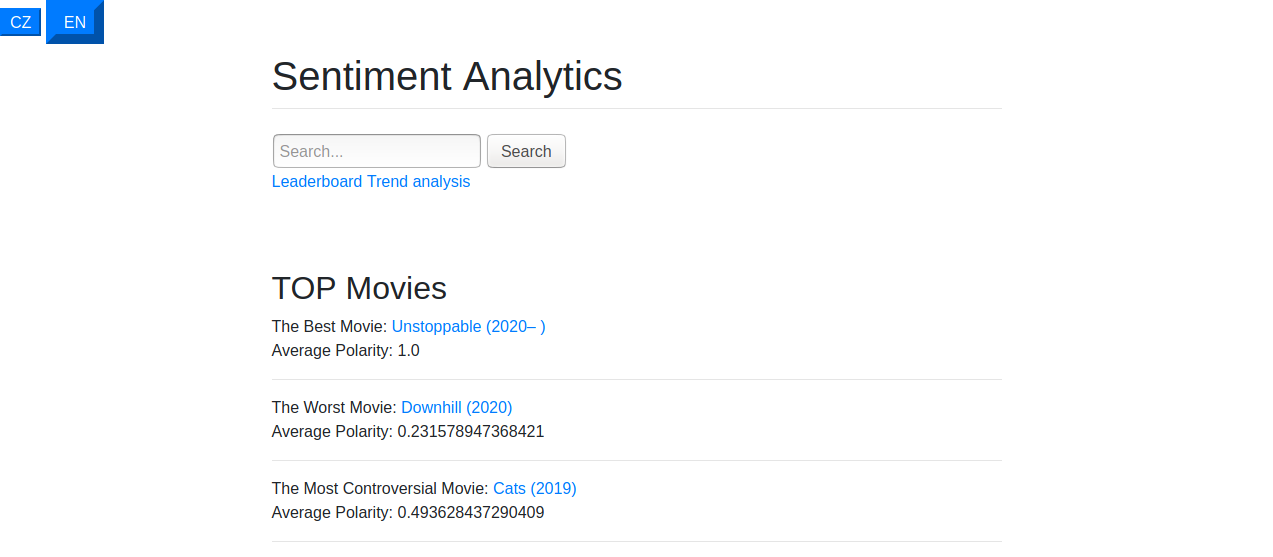
\includegraphics[width=\textwidth]{homepage.png}
\caption{Domovská stránka webového rozhraní.}
\end{figure}
\FloatBarrier
Obrázek \ref{homepg} ukazuje vzhled domovské stránky. V levém horním rohu jsou tlačítka pro přepnutí jazyka stránek. Celý systém je implementován pro češtinu i angličtinu, proto je i~zde možnost přepínat jazyky. Přepnutí jazyka změní text na stránkách i data dotazovaná z databáze. Stránky přepnuté do češtiny využívají pouze data získaná z českých zdrojů.

Domovská stránka nabízí vyhledávací okno, vyhledávat se dají tituly podle jejich názvu. Výsledkem vyhledávání je seznam všech titulů, jejichž název obsahuje hledaný výraz. Ke každému z vyhledaných filmů je připsána jeho popularita (celkový počet recenzí v databázi). 

Dále je na stránce tlačítko pro přejití na žebříček titulů, pod ním je seznam top filmů. Tlačítko pro přejití na stránku analýzy trendů je přítomno pouze pokud je stránka přepnuta do angličtiny. Analýza trendů se pro češtinu neprovádí.  

\pagebreak
\subsection{Žebříček}
\FloatBarrier
\begin{figure}[!htb]
\label{leaderb}
\centering
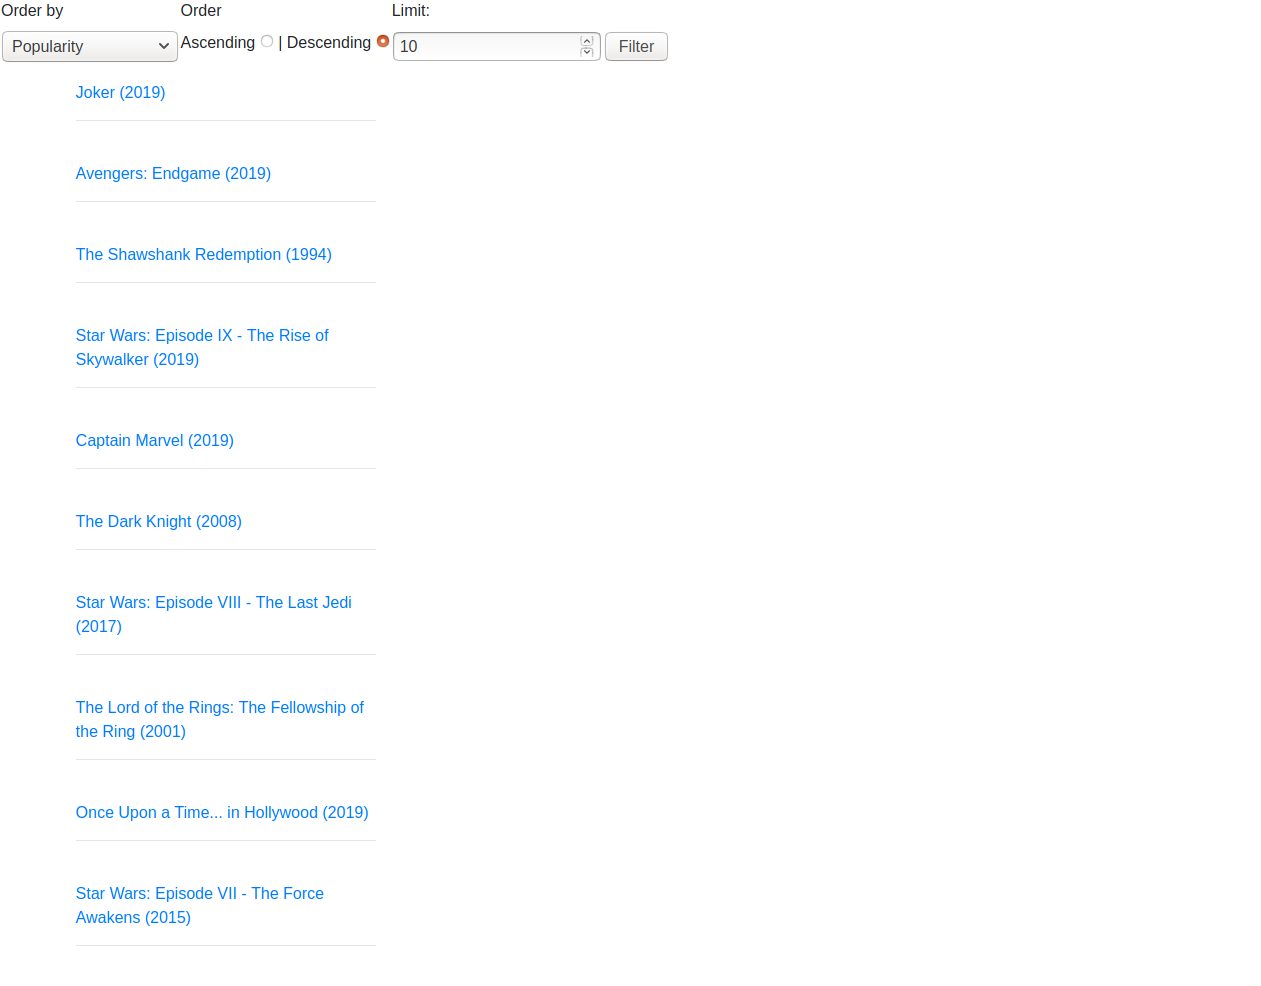
\includegraphics[width=\textwidth]{leaderboard.png}
\caption{Žebříček nejlepších / nejhorších titulů.}
\end{figure}
\FloatBarrier
Jak je vidět na obrázku \ref{leaderb}, žebříček nabízí limitovaný seznam titulů seřazených vzestupně nebo sestupně podle jednoho z následujících parametrů (hodnoty z tabulky movies):
\begin{itemize}
  \item Průměrná polarita.
  \item Průměrný počet hvězd.
  \item Popularita.
  \item Průměrné hodnoty jednotlivých aspektů. 
\end{itemize}
Celkově je tedy možnost řadit tituly podle jednoho z osmi parametrů. Limit počtu zobrazených titulů je samozřejmě nastavitelný. 

\pagebreak
\subsection{Detail filmu}
\label{moviedetail}
\FloatBarrier

\begin{figure}[!htb]
\label{movied}
\centering
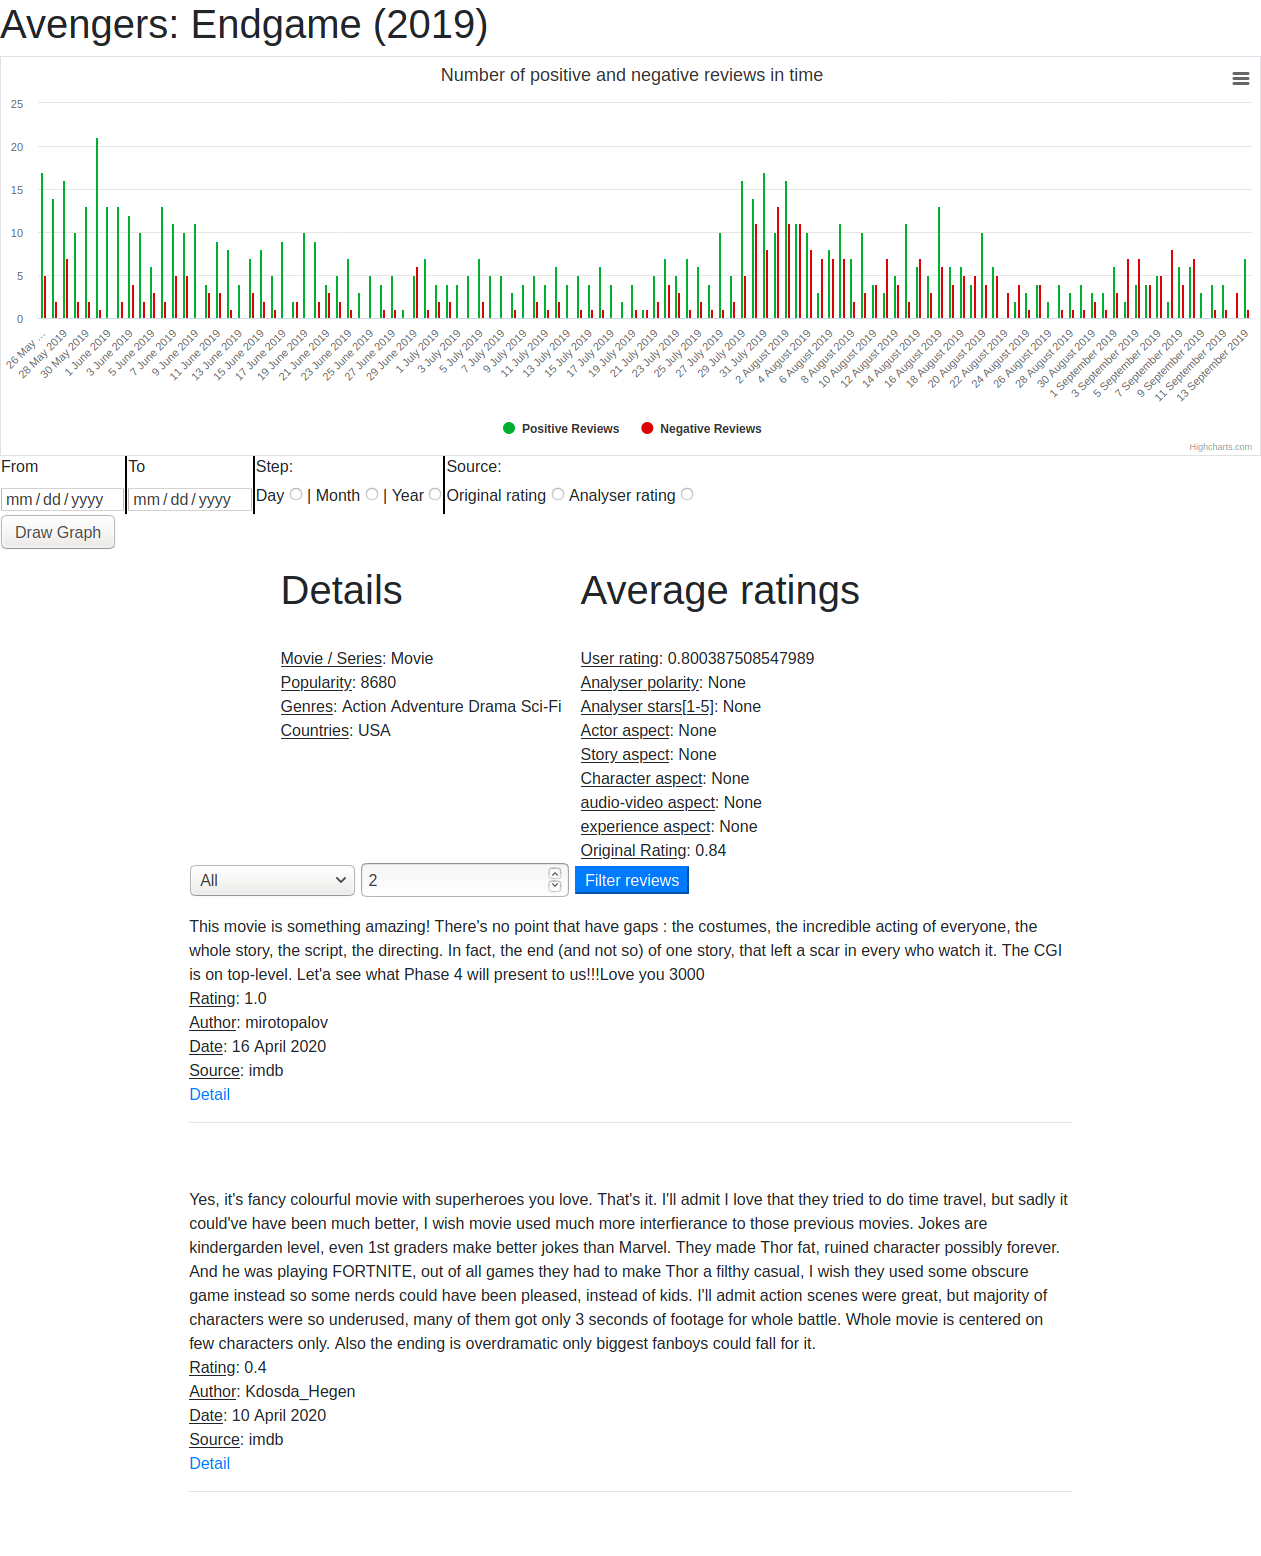
\includegraphics[width=\textwidth]{movie_detail.png}
\caption{Detailní informace o filmu.}
\end{figure}
\FloatBarrier
Stránka zobrazující detaily o filmu je na obrázku \ref{movied}. V horní sekci stránky je graf zobrazující názor na titul v čase. Nastavením grafu lze měnit časový interval i jeho krok. Dále lze nastavit zdroj názorů na daný film, první možností je originální hodnocení uživatelů, druhou možností jsou výsledky polaritní analýzy.

Ve spodní sekci stránky jsou jednotivé recenze k danému filmu. Ty je možné filtrovat podle aspektu o kterém recenze hovoří. Opět je možnost limitovat maximální počet zobrazených recenzí. 

\subsection{Detail recenze}
\FloatBarrier
\begin{figure}[!htb]
\label{reviewd}
\centering
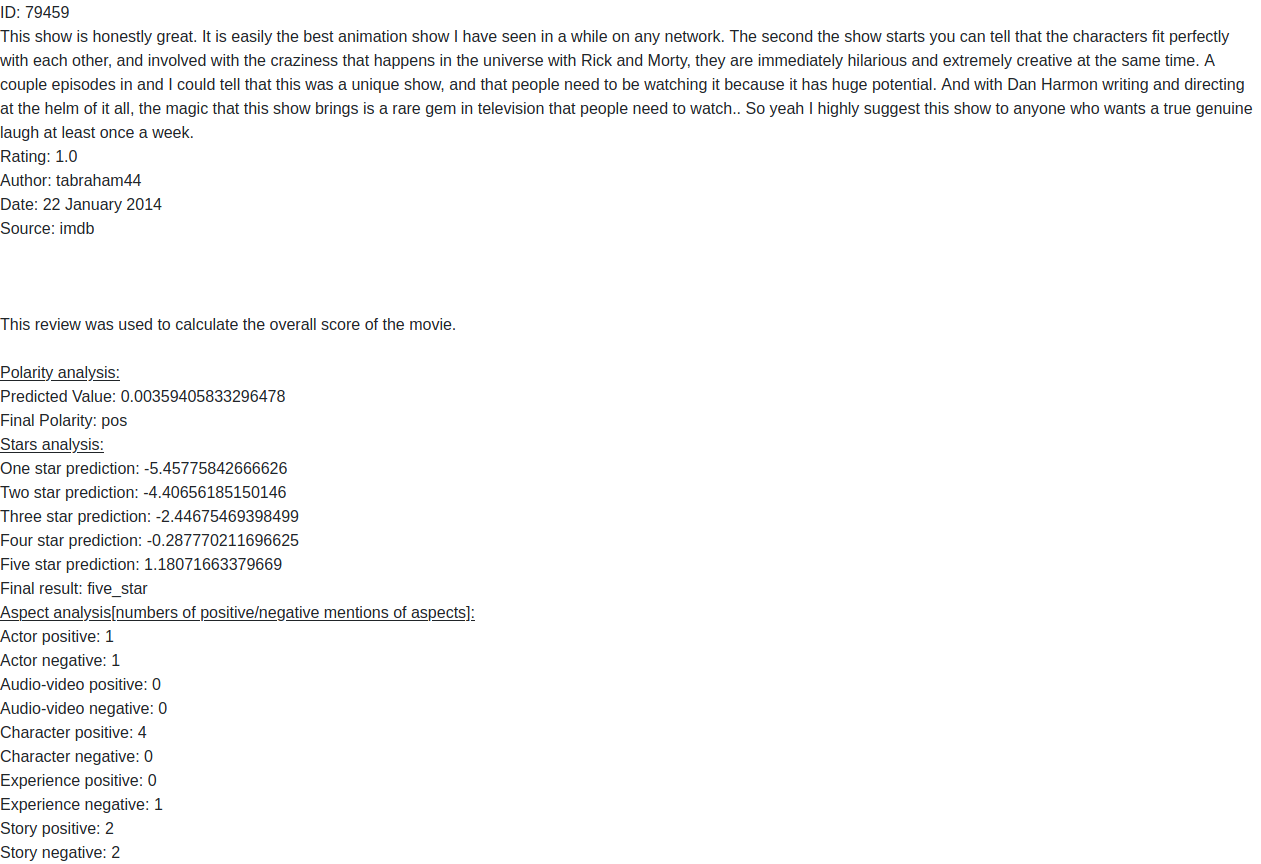
\includegraphics[width=\textwidth]{reviewdetail.png}
\caption{Detailní informace o recenzi.}
\end{figure}
\FloatBarrier
Stránka detailů recenze je na obrázku \ref{reviewd}. Obsahuje všechny detaily týkající se dané recenze. Pokud byla recenze již analyzována, obsahuje také výsledky analýz.

\pagebreak
\subsection{Analýza trendů}
\FloatBarrier
\begin{figure}[!htb]
\centering
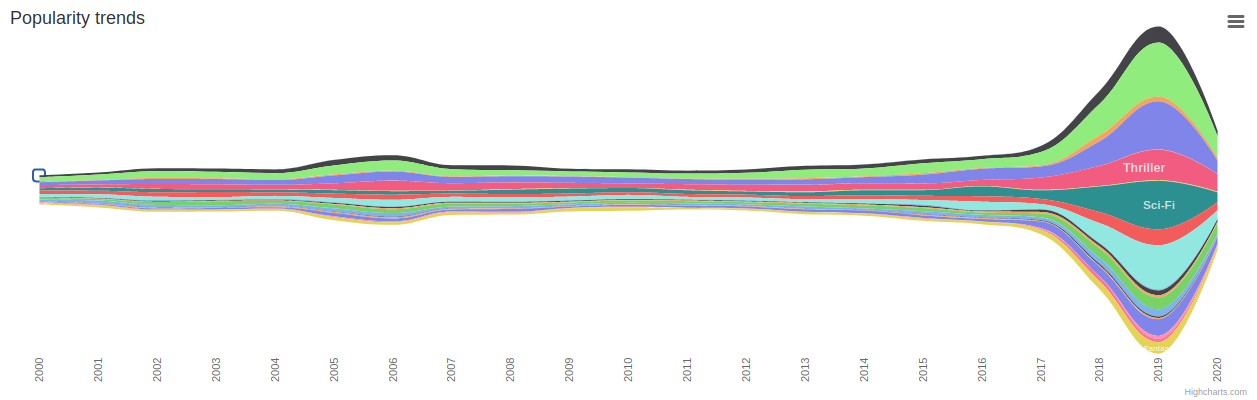
\includegraphics[width=\textwidth]{genres.png}
\label{trend}
\caption{Graf trendů popularity.}
\end{figure}
\FloatBarrier
Stránka obsahuje graf trendu popularity v čase (obrázek \ref{trend}). Popularita je zde definována jako celkový počet recenzí v databázi. Vykreslování grafu je opět nastavitelné. Krok grafu je vždy jeden rok, trendy nemá moc smysl sledovat v menším měřítku. Popularitu je možné sledovat podle typu titulu (film / seriál), podle žánru a podle země původu.

